% Section 2: Methodology
\section{Methodology}
\label{sec:methodology}

This section details the proposed methodology for Point-of-Interest (POI) category classification and next-POI prediction using a MTL approach. We first describe the generation of POI embeddings and the preparation of data for both tasks. Subsequently, we present the architectures of the single-task baselines, which are also used as task-specific heads within our MTL framework. Finally, we elaborate on the proposed MTL architecture, including the hard parameter-sharing strategy and the Nash-MTL optimizer employed for gradient aggregation.


\subsection{POI Embeddings and Data Preparation}
\label{subsec:embeddings_data_prep}

This work computes POI embeddings using graph attention convolution along with contrastive learning based on Deep Graph Infomax (DGI). These embeddings are the input for the MTL model discussed in Section \ref{sec:method:mtl}.

\subsubsection{POI Embeddings}

A point of interest is defined as a tuple $\langle id, lat, long, cat \rangle$, where $id$ serves as a unique identifier, $lat$ and $long$ represent its coordinates, and $cat$ denotes its category, such as restaurant or pharmacy. A place suffers from complementarity effect \cite{du2019beyond}, implying that a location is affected by its neighbors (e.g. leisure zones are often near residential districts). Hence, we propose a graph-based contrastive method to capture this spatial locality behavior, generating a POI embedding to serve as input to our MTL model.

To capture the spatial locality and capture neighborhood information, we model the weighted graph $G(V, E)$ as a Delaunay Triangulation, where each vertex $v \in V$ represents a POI and edge $e_{ij} \in E$ defines the connection between POI $p_i$ and a POI $p_j$. Besides that, following \cite{huang2022estimating} the weight of an edge $e_{ij}$ is defined as $w_{ij} = \log((1+D^{1.5}/1+d_{ij}^{1.5}))$, where D is the diagonal length of bounding box that encloses the coordinates of POIs, and $d_{ij}$ is the geodesic distance between $p_{i}$ and $p_{j}$. The node feature matrix is based on category one-hot encoding of each POI, represented by $X \in \mathbb{R}^{n_c}$, where $n_c$ is the number of possible categories.

Therefore, to encode the Delaunay graph we apply a graph attention convolution layer \cite{velivckovic2017graph}, yielding an embedding $h_i \in \mathbb{R}^{d}$, where $d$ is the dimension of the output. Moreover, we utilize a Deep Graph Infomax (DGI) \cite{velivckovic2018deep} as a contrastive learning method to maximize the mutual information between local representations (node embeddings) and the global graph embedding compared to a corrupted version of a graph, which is guided by the Equation \ref{eq:loss}.
%
\begin{IEEEeqnarray}{rCl}
  \mathcal{L}
  &=& \frac{1}{2|V|}\Bigl(
        \sum_{i=1}^{|V|}
          \mathbb{E}_{(X,G)}
          [\log \mathcal{D}(\vec{h}_i,\vec{s})] \nonumber\\
  &&\quad {}+
        \sum_{j=1}^{|V|}
          \mathbb{E}_{(\tilde{X}, G)}
          [\log (1-\mathcal{D}(\tilde{\vec{h}}_j,\vec{s}))]\Bigr)
  \label{eq:loss}
\end{IEEEeqnarray}
%
where $X$ and $G$ denote the positive samples for the node feature matrix and graph adjacency, respectively, while $\tilde{X}$ is the corrupted version of the feature matrix. To corrupt the features, we employ a random shuffling method. Additionally, $\vec{s}$ is the global graph embedding derived by applying global mean pooling to the embedding matrix $H = [h_i, h_{i+1}, \ldots, h_{n}]$ in our model. Moreover, $\mathcal{D}$ is a discriminator that differentiates each positive example from its corrupted version, learning from their dissimilarities; in our POI Embedding, this discriminator is implemented as a linear model.

\subsubsection{Data Processing for POI Category Classification}
Each POI is represented by its 64-dimensional DGI embedding $\mathbf{e}\!\in\!\mathbb{R}^{64}$.  
The dataset therefore consists of pairs $(\mathbf{e},\,c)$, where $c$ is the POI’s ground-truth category to be predicted.

\subsubsection{Data Processing for Next-POI Category Prediction}
This task predicts the category of the next POI a user will visit from their recent check-in history.

\begin{enumerate}
  \item \textbf{Trajectory building.}  Check-ins (user, POI, timestamp) are ordered chronologically per user; users with fewer than five visits are discarded.
  \item \textbf{Sequence extraction.}  From each trajectory we draw non-overlapping windows of length $L_h\!=\!9$: $(p_1,\dots,p_9)$ as context and $p_{\text{target}}$ as the next POI.
  \item \textbf{Feature/label construction.}
    \begin{itemize}
      \item The input is the concatenation of the 64-dimensional embeddings of $p_1$–$p_9$, yielding a $9\!\times\!64=576$-dim vector.  
            Histories shorter than nine are padded by a special POI whose embedding is $\mathbf{0}$.
      \item The label is the category of $p_{\text{target}}$.
    \end{itemize}
\end{enumerate}

This format allows the model to infer the category of the next POI solely from the embeddings of the previous visits.

%
% Multi-Task Learning Architecture
%
\subsection{Multi-Task Learning Architecture}
\label{sec:method:mtl}

Our proposed Multi-Task Learning (MTL) architecture, depicted in Figure~\ref{fig:arch}, is built upon a hard parameter-sharing scheme for the joint training of POI Category Classification and Next-POI Prediction. This design integrates Feature-wise Linear Modulation (FiLM) layers to condition the shared representations, a technique aimed at modulating task interactions and mitigating negative transfer \cite{perez2018film, standley2020tasks}.

\paragraph*{Architecture Overview}
Input features for POI Category Classification ($\mathbf{x}^{(c)}$) and Next-POI Prediction ($\mathbf{x}^{(n)}$) are first processed by separate, task-specific encoders. These encoders, implemented as MLPs, map the raw input features into a shared latent space of dimension $d_{\mathrm{shared}}$.

\paragraph*{Feature-wise Linear Modulation (FiLM)}
To allow for task-specific adaptation within the shared pathway, we employ FiLM layers \cite{perez2018film}. A unique, learnable task embedding $\mathbf{e}_{t}$ for each task $t$ is used to generate a scaling vector $\gamma_{t}$ and a shifting vector $\beta_{t}$. These vectors modulate the encoded features $\mathbf{h}_{\mathrm{enc}}^{(t)}$ from each task-specific encoder:
$$
\mathrm{FiLM}(\mathbf{h}_{\mathrm{enc}}^{(t)} \,|\, \mathbf{e}_{t}) = \gamma_{t} \odot \mathbf{h}_{\mathrm{enc}}^{(t)} + \beta_{t}
$$
This lightweight operation conditions the features before they enter the fully shared layers of the network.

\paragraph*{Shared Processing Layers}
The FiLM-modulated representations are processed by a sequence of shared layers. This module begins with a linear transformation followed by a LeakyReLU activation, LayerNorm, and dropout, and continues through $L_{\mathrm{shared}}$ residual blocks. This hard parameter-sharing approach regularizes the model by forcing it to learn a common, robust feature representation for both tasks \cite{baxter2000model}.

\paragraph*{Task-Specific Heads}
Finally, the processed shared representations are passed to dedicated, unshared task-specific heads, as detailed in Section~\ref{sec:method:single_task_heads}. These heads generate the final predictions for each task, allowing for specialized output generation and isolated gradient computation during backpropagation.

\paragraph*{Rationale for Hard Parameter Sharing}
The choice of hard parameter sharing is motivated by its efficiency and regularization benefits, which are critical for our target application. This approach is supported by several factors:
\begin{itemize}
    \item \textbf{Computational Efficiency:} Unlike soft-sharing methods that often introduce task-specific parameters and increase computational overhead, hard sharing maintains a compact model. This is crucial for deployment on resource-constrained edge devices (e.g., NVIDIA Jetson platforms).
    \item \textbf{Implicit Regularization:} By constraining the hypothesis space, hard sharing acts as a regularizer, often leading to more generalizable models, especially when tasks are related \cite{ruder2017sluice}. Seminal work by Caruana demonstrated significant error reduction with this approach \cite{caruana1997multitask}.
    \item \textbf{Empirical Performance:} In practice, hard parameter sharing frequently matches or exceeds the performance of more complex architectures on many benchmarks, while offering faster training and inference \cite{standley2020tasks}.
\end{itemize}
This architecture strategically balances model capacity with knowledge transfer, prioritizing efficiency for potential real-time recommendation scenarios.

\begin{figure*}[htbp]
    \centering
    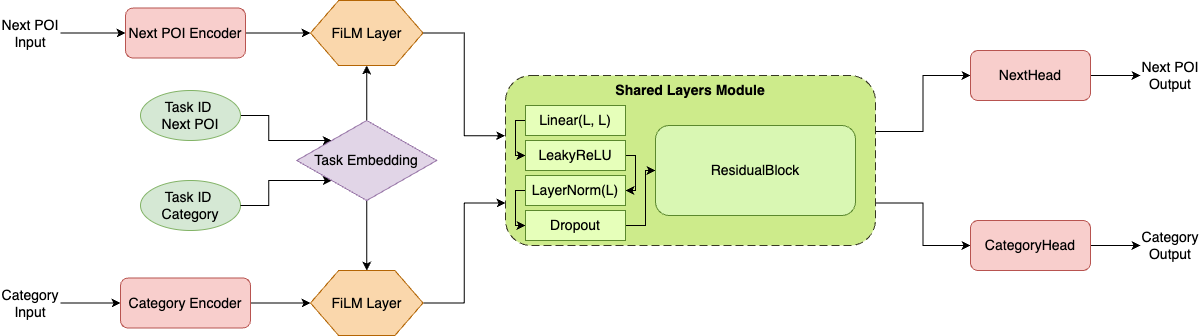
\includegraphics[width=\textwidth]{imgs/mtlnet_poi.drawio.png}
    \caption{The proposed Multi-Task Learning (MTL) architecture. Task-specific encoders process inputs for POI Category Classification and Next-POI Prediction. Feature-wise Linear Modulation (FiLM) layers adapt these features using learnable task embeddings. The modulated representations are then processed by a shared path of residual blocks. Finally, dedicated task-specific heads generate the respective outputs.}
    \label{fig:arch}
\end{figure*}
%
% Nash–MTL Optimizer
%
\subsection{Nash–MTL Optimizer}\label{sec:nash_mtl}

MTL necessitates a unified update direction that benefits all tasks, even when their gradients conflict. Nash-MTL formulates this as a cooperative $K$-player bargaining game\cite{nash}, where each task acts as an "agent" seeking to maximize its utility (loss reduction). The optimizer selects a step that is (i) beneficial to all tasks, (ii) scale-invariant to arbitrary loss re-weightings, and (iii) proportionally fair, ensuring no alternative direction increases one task's utility without decreasing the product of all utilities\cite{nash}. The unique solution satisfying these axioms is the Nash Bargaining Solution (NBS). This approach allows Nash-MTL to "negotiate" at each iteration, yielding a compromise descent direction that improves every loss while maximizing the joint progress of the entire system.

\paragraph*{Formal Formulation.}
Given task-specific objectives $\{\mathcal{L}_k(\boldsymbol{\theta})\}_{k=1}^{K}$ and their gradients $\mathbf{g}_k=\nabla_{\!\boldsymbol{\theta}}\mathcal{L}_k$ at current parameters $\boldsymbol{\theta}$, Nash-MTL frames gradient aggregation as a bargaining game to determine the common update direction \cite{nash}. The utility for each task $k$ is its signed improvement, $u_k(\Delta\boldsymbol{\theta})=\mathbf{g}_k^{\!\top}\!\Delta\boldsymbol{\theta}$, where $\Delta\boldsymbol{\theta}$ is the parameter update within an $\varepsilon$-ball \cite{nash}. The NBS is found by maximizing the weighted geometric mean of utilities:
\begin{equation}
\Delta\boldsymbol{\theta}^{*}\;=\;\argmax_{\Delta\boldsymbol{\theta}\in\mathcal{B}_\varepsilon}
\sum_{k=1}^{K}\!\log\!\bigl(u_k(\Delta\boldsymbol{\theta})\bigr)
\quad\text{s.t. }u_k(\Delta\boldsymbol{\theta})>0,\;\forall k.
\label{eq:nbs_objective}
\end{equation}
By setting $\Delta\boldsymbol{\theta}=\sum_{k}\alpha_k\mathbf{g}_k$ with positive weights $\boldsymbol{\alpha}$, the solution simplifies to solving the nonlinear system $\bigl(\mathbf{G}^{\!\top}\mathbf{G}\bigr)\boldsymbol{\alpha} \;=\; \boldsymbol{\alpha}^{-1}$ \cite{nash}, where $\mathbf{G}=\bigl[\mathbf{g}_1\,\ldots\,\mathbf{g}_K\bigr]$ \cite{nash}. The parameter update is then $\boldsymbol{\theta}^{(t+1)} =\boldsymbol{\theta}^{(t)}-\eta\,\mathbf{G}\boldsymbol{\alpha}$, with $\eta$ chosen to ensure monotonic loss decrease and convergence to a Pareto-stationary point \cite{nash}.

\paragraph*{Practical Aspects.}
Nash-MTL is architecture-agnostic and requires only two matrix-vector products per iteration. Its reliance on gradient signs rather than scales inherently balances heterogeneous tasks without manual re-weighting. For efficiency, task weights can be updated less frequently, significantly reducing runtime while maintaining performance~\cite{nash}.


\paragraph*{Parameter Partition.}
In our model (Figure~\ref{fig:arch}), we explicitly expose two disjoint parameter sets:
\[
\resizebox{\linewidth}{!}{$%
  \begin{aligned}
    \Theta_{\text{shared}}   &= \{\texttt{task\_emb},\texttt{film},\texttt{shared\_layers}\},\\
    \Theta_{\text{specific}} &= \{\texttt{category\_encoder},\texttt{next\_encoder},
                                 \texttt{CategoryHead},\texttt{NextHead}\}.
  \end{aligned}
$}
\]
This partition enables independent learning-rate scheduling or regularization if domain shifts between tasks emerge during fine-tuning.

The Nash-MTL optimizer was employed for its ability to aggregate tasks gradients in a balanced and principled manner, formulating the optimization process as a bargaining problem and aiming for joint progress across all tasks. In our evaluation, Nash-MTL was compared with different strategies, including PCGrad~\cite{yu2020pcgrad}  and an approach with no optimizer. Among these, it was found that Nash-MTL consistently yielded a better overall performance of the MTL model, with a lower combined multi-task loss, which supported our decision to adopt it as our choice of optimizer.
